\documentclass[a4paper,12pt]{article}
\usepackage{graphicx}
\usepackage[hidelinks]{hyperref}
\usepackage{listings}
\setcounter{tocdepth}{1}
\usepackage{float}
\begin{document}
\begin{center}

\Huge\textbf{Architecture Requirements\\}
																											
\vspace{2 cm}

\LARGE\textbf{Group Name:} Group 7\_a\newline
 
\vspace{0.5 cm}
\begin{tabular}{lr}
Roger Tavares&10167324\\
Thinus Naude&13019602 \\
Kabelo Kgwete&11247143\\
Sylvester Mpanganer&11241617\\
Maphuti Setati&12310043\\
Ruth Ojo&12042804\\
Axel Ind&12063178\\
Lindelo Mapumulo&12002862\\
Maria Qumalo&29461775\\
\end{tabular}

\vspace{1cm}
\textbf{Git repository link:\\}
\url{https://github.com/thinusn/COS301MiniProjectArchitectureRequirements}

\vspace{1cm}
\textbf{Date:} 04 March 2015
\end{center}

%-----------------TABLE OF CONTENT-----------------
\newpage
\tableofcontents


%-----------------BASIC INTRODUCTION-----------------
\newpage
\setlength{\voffset}{-3cm}
This document contains specifications of the software architecture 
\\requirements. This is the infrastructure upon which the application
\\ functionality will be developed. The following non-functional
\\ requirements are addressed in depth with supporting diagrams
\\(when necessary):

\begin{itemize}
	\item Access and Integration requirements.
	\item Architectural responsibilitie.
	\item Quality requirements.
	\item Architecture constraints as specied by the client. 
\end{itemize}

%-----------------PARTS TO EDIT-----------------
\newpage
\setlength{\voffset}{-3cm}

%-----------------MARIA AND ROGER-----------------
\section{Access and integration requirements}
\subsection{Access channels}
\subsubsection{Human access channels} %---MARIA
\subsubsection{System access channels}%---ROGER


%-----------------SYLVESTER AND MAPHUTI-----------------
\subsection{Integration channels}

%-----------------SYLVESTER AND MAPHUTI-----------------
\section{Architectural responsibilities}

%-----------------THIUNS AND KABELO-----------------
\section{Quality requirements}
%-----------------THIUNS -----------------
\subsection{Scalability}
\begin{itemize}
	\item The Buzz Space discussion board should allow for more than a million concurrent users.\footnote{Communicated to us via email correspondence with Mrs. Vreda Pieterse}
	\item This scalability will be achieved by running many instances of the application over a cluster of servers or instances. This can be achieved by using a cloud hosting platform such as Amazon Web Services.
	\item There will need to be a load balancer in order to ensure every request is handled by a server that is not over or at capacity. If the limit for a server is reached (user configurable) a new instance needs to be created to handle the number of increased requests. If the amount of requests are at or below a certain limit (user configurable) the amount of instances needs to be reduced.
	\item In order to facilitate persistent storage to th database connections need to be grouped and accessed via a central channel. 
	\item Caching of objects/frequently requested database queries will be facilitated by a separate module. The caching will interface with the system as well as the database to ensure frequent objects and queries aren't repeated or fetched over and over again wasting system resources.
	\item The Scalability discussed here can be seen as an illustration in Figure ~\ref{fig:scalability}.
	\begin{figure}[H]
		\centering
		\fbox{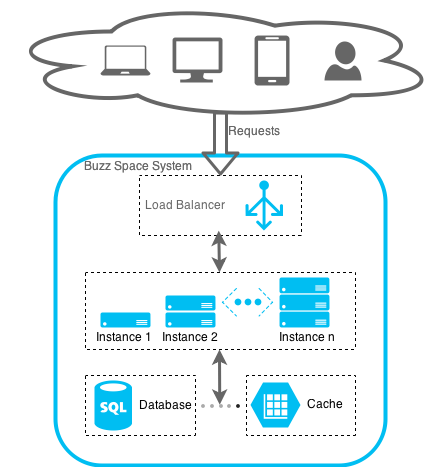
\includegraphics[width=1.0\textwidth]{Scalability.png}}
		\caption{How the system architecture can be set-up to allow many concurrent connections.}
		\label{fig:scalability}
	\end{figure}
\end{itemize}
%-----------------THIUNS -----------------
\subsection{Performance requirements}
\begin{itemize}
	\item The system needs to be hardware and software fault tolerant (to a certain degree). The system needs to continue working/running as intended but possibly at a reduced level, rather than breaking/stopping completely.
	\item The system needs to be responsive. The time it takes for a request to be sent back to a user should be minimized. 
	\item The UI presented to the user needs to be clean, dynamic and use minimal resources. An example would be to use minified JavaScript files and compressed images.
	\item The performance of the system needs to be optimal, memory or processor intensive tasks should run/execute when there are the least number of active users in order to minimize the impact these tasks will have on performance.
	\item The system needs to have a coping mechanism when there is a sudden change of environment. (E.g. can handle 100 connections suddenly there is 10000 connections). Performance will suffer if this is not taken into consideration.
	\item The system should deliver intermediate results or updates to the user when executing a request. For instance, a web page that submits a form via AJAX can have a status/busy indicator to let the user know his/her request is being processed.
\end{itemize}
%-----------------THIUNS -----------------
\subsection{Maintainability}
\begin{itemize}
	\item Dependency injection will be used to fully decouple the implementation classes. Dependencies are purely on contracts (interfaces) and not on classes.
	\item The system needs to be capable of improvement in functionality by the addition or replacement of components.
	\item The system needs to easily facilitate:
	\begin{itemize}
		\item Detection of problems/errors and their cause(s)
		\item Repair or replacement of faulty or deprecated modules without having to replace still working modules.
		\item Prevention of total breakdowns.
		\item Adaptability to new requirements.
		\item Easy deployment of modifications to improve performance or other attributes.
	\end{itemize}
	\item Throughout the implementation stage strict coding standards/guidelines should be followed. This will keep the code code clean, consistent, and easy to read. See Figure ~\ref{fig:posibCodeStyle} for an example of a suggested code style.
	\item For easy reference source code documentation will be generated by the Javadoc program.
	\begin{figure}[H]
		\fbox{\lstinputlisting[language=Java]{style.java}}
		\caption{Possible style guide for code to be used in the project.}
		\label{fig:posibCodeStyle}
	\end{figure}
\end{itemize}
%-----------------THIUNS -----------------
\subsection{Reliability and Availability}
\begin{itemize}
	\item The availability of the system needs to be as high as possible if a breakdown occurs, the system needs to recover by itself. 
	\item The system needs to allow multiple or different database connections
	\item All components of the system need to have redundancies built in.
	\begin{itemize}
		\item If the database connection fails, a connection to the redundant database needs to be established. 
		\item If a server instance fails, the error needs to be logged and the server should restart and try to recover from the breakdown. 
		\item If a data-centre where some of the system instances are hosted goes down the system should only suffer temporarily. The instances need to spread across multiple datacentres or locations. 
	\end{itemize}
	\item The reliability of the system should be tested by using unit tests and acceptability testing.
	\item The system should allow for a notification to be send to a user, if their request has failed or the delivery there of has failed. 
\end{itemize}
%-----------------THIUNS -----------------
\subsection{Security}
\begin{itemize}
	\item The system will interface with LDAP to provide authentication.
	\item All communication with the database needs to be handled over an encrypted connection.
	\item The system will need to support encryption (https) via SSL.
	\item All requests will be logged and if required audited to verify no unauthorised access to the system resources has been gained.
	\item The system will monitor all service requests in Buzz, irrespective of the channel through which they are requested. These requests will be validated by the "Authorization Interceptor" module which checks whether the user is authorized to use the service that they requested. 
	\item At all times the system needs to minimize the chance of malicious or accidental actions by unauthorised users. 
	\item The system needs to prevent disclosure or loss of information. 
	\item The system needs to be built to withstand common malicious attacks such as SQL injection and cross-site scripting.
	\item The system needs to be able to detect and mitigate Denial of service (DoS) attacks, either by using a hardware of software approach. 
\end{itemize}
%-----------------KABELO-----------------
\subsection{Monitorability and Auditability}
%-----------------KABELO-----------------
\subsection{Testability}
%-----------------KABELO-----------------
\subsection{Usability}
%-----------------KABELO-----------------
\subsection{Integrability}

%-----------------RUTH AND LINDELO-----------------
\section{Architecture constraints}
\end{document}